\documentclass{scrbook}

\usepackage{graphicx}

\usepackage{wrapfig}

\usepackage{multicol}

\title{Patterns}
\author{Firstname1 Lastname1 \and Firstname2 Lastname2 \and Firstname3
Lastname3 \and Firstname4 Lastname4}
\date{\today}


\begin{document}
\frontmatter
\maketitle
\tableofcontents
\mainmatter
\part{Architectural Patterns}
\chapter{Pipes and Filters}
\chapter{Blackboard}
\chapter{Broker}

%Groups I and H
\chapter{Presentation-Abstraction-Control}

\section{Example}



\section{Context}

\section{Problem}

\begin{multicols}{2}
 



In interactive systems multiple agents work at the same time on separate parts of the same project
(horizontal decomposition). Also, some agents work closer with the database and some of them
closer with the users (vertical decomposition).


\begin{center}
 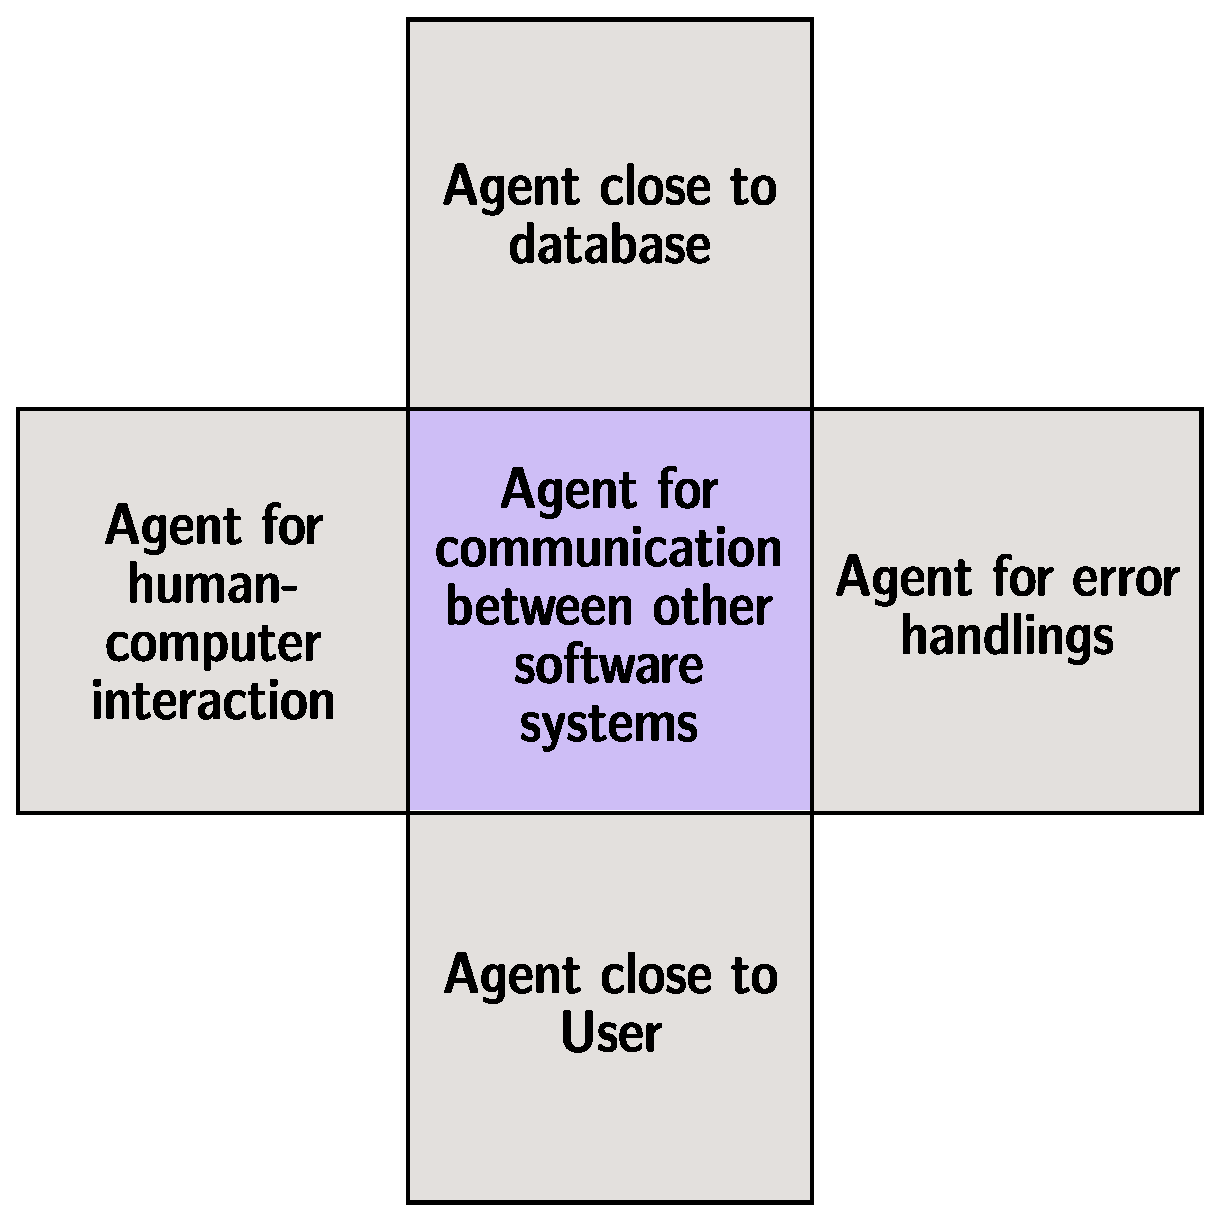
\includegraphics[width=0.4\textwidth]{./pics/problem.eps}\end{center}
 % problem.eps: 0x0 pixel, 300dpi, 0.00x0.00 cm, bb=0 -1 570 570

\end{multicols}

\section{Solution}

\section{Structure}

\section{Dynamics}

\section{Known Uses}

%end Groups I and H


\chapter{Microkernel}
\chapter{Reflection}

\end{document}
